\documentclass[thesis=M,english,hidelinks]{FITthesis}[2018/06/01]

\usepackage[utf8]{inputenc}

\usepackage{graphicx}

\usepackage{dirtree}

\department{Department of Theoretical Computer Science}
\title{Fine-tuning LLVM optimizations}
\authorGN{Tomáš} %author's given name/names
\authorFN{Drbota} %author's surname
\author{Tomáš Drbota} %author's name without academic degrees
\authorWithDegrees{Bc. Tomáš Drbota} %author's name with academic degrees
\supervisor{doc. Ing. Ivan Šimeček, Ph.D.}
\acknowledgements{TODO}
\abstractEN{Modern compilers provide a wide range of different optimizations in an effort to increase the performance of the resulting program. Many of them already offer ways to customize the amount of optimization - for example -O flags in GCC, compiler arguments (e.g. -finline-functions in Clang) or in-line attributes (e.g. \#pragma unroll), but the overall granularity of these options is low.
	
The purpose of this work is to investigate options for further customizing the execution of transformation passes in an optimizing compiler and comparing the results to automatically optimized code. The intent is to ensure there are ways for the user to be able to specifically declare which transformations should or should not be used in a given scope. Implementation is done using LLVM and its C/C++ frontend, Clang.}
\abstractCS{TODO}
\placeForDeclarationOfAuthenticity{Prague}
\keywordsCS{Replace with comma-separated list of keywords in Czech.}
\keywordsEN{llvm, clang, compiler, transformation, optimization}
\declarationOfAuthenticityOption{5}
% \website{http://site.example/thesis} %optional thesis URL

\begin{document}

\setsecnumdepth{part}
\chapter{Introduction}
In today's age of smartphones and other portable electronic devices capable of connecting to the internet, nearly everyone has access to a huge library of various media, including music and other audio. However, to transmit or store all of this data in its raw uncompressed form, a large amount of bandwidth and storage would be required. It is for that reason that we must employ some sort of compression.

Lossy audio codecs such as MP3, AAC, AC3, Vorbis, Opus etc. have been prevalent in this field as they are capable of compressing an audio signal into even a tenth of its size, without a perceivable difference in quality (to our ears, at least).

As such, this thesis will look into using Non-negative matrix factorization as a possible method for lossy compression of audio. It has been employed before for audio analysis, but works describing its applications for compression of audio specifically are limited.

First, we will have a look at what even is digital audio and important terms surrounding it. We will explore how it works, how is it recorded and stored in a computer and also what concerns go into analysing and compressing it.

Then, in chapter 3, non-negative matrix factorization is defined and described. We will talk about what it is, what is it realistically used for, how to use and implement it, and lastly its applications in the field of digital audio.

After that, we finally get to data compression. State of the art lossy audio codecs will be examined along with some lossless encodings that will be necessary later. Existing research into audio compression using NMF will also be summarized.

In chapters 5 and 6, I design and implement an NMF encoder and decoder (called ANMF). There are three different variants depending on what's being compressed - \emph{ANMF-RAW} for encoding raw audio, and \emph{ANMF-MDCT} along with \emph{ANMF-STFT} for encoding properly pre-processed audio. The file structure along with all the implementational details including used libraries will be described in great detail.

And finally, we take the implementation and evaluate the results. Using GstPEAQ as an objective measuring method, we compare our implementation to some of the reference codecs, namely MP3 and Opus, and draw conclusions from the results.


\addtocontents{toc}{\setcounter{tocdepth}{2}}

\setsecnumdepth{all}
\part{Background}
\chapter{LLVM architecture}
LLVM \cite{Lattner:MSThesis02}, formerly known as \emph{Low-Level Virtual Machine} is "a collection of modular and reusable compiler and toolchain technologies" \cite{llvm_web}. Originally intended as a compiler infrastructure well-suited for modern programming languages, it has since grown into an umbrella term for a decently large group of sub-projects, intended for building everything related to compilers, that is frontends, backends, optimizers, Just-In-Time compilers etc. Some of these sub-projects will be discussed later in the chapter.

Today, LLVM is a popular choice for TODO

This work will be using LLVM and its toolset exclusively.

\section{Structure}
Written in C++, at its core LLVM uses a classical three phase compilation process \cite{Lattner:LLVM_Design}, popular for static compilers. These three phases are namely the frontend, optimizer, and backend.

The frontend is responsible for parsing and validating the source code, generally producing some sort of intermediate form. The optimizer then takes this form, and does various transformations to improve the code's running time, and is mostly independent of the target. Finally, the backend generates actual machine code specific to the architecture.

The main benefit of this design is that a programmer writing source code doesn't need to worry about architecture specific assembly code or optimizations, and one code should work the same on every platform supported by the backend.

\section{Intermediate Representation}
As I have mentioned in the previous section, all three phases during compilation work with some sort of intermediate code. In LLVM this internal assembly language is called \emph{Intermediate Representation} \cite{llvm_ir} (\emph{LLVM IR} for short, or just \emph{IR}), and it's arguably one of the most important parts of LLVM.

LLVM IR is a well specified SSA (Static Single Assignment) based representation that provides type safety and various low-level operations. It is the only interface to LLVM's optimizer and is used throughout all phases of LLVM's compilation process.

There are three different forms of LLVM IR, all of which are equivalent:
\begin{itemize}
	\item in-memory compiler IR
	\item on-disk bitcode representation (e.g. for JIT)
	\item a human readable assembly representation
\end{itemize}

The ability to have human readable IR is going to be extremely helpful, as it allows the developer to write or edit arbitrary IR and compile it to an executable file. This is difficult to do with other compilers, e.g. GCC's \emph{Gimple} only allows printing its intermediate form, but you cannot trivially edit and compile it to a functioning program.

I am not going to go into large detail here regarding the exact structure of a well-formed IR module, but having an overview is going to be necessary for understanding the implementation.

\subsection{Module}
An LLVM program is composed of one or more modules, which represent a translation unit of the input files. Modules consist of functions, global variables and symbol table entries. These module files can be further merged together (along with symbol resolution etc.) using the LLVM linker, but that's not required.

Incidentally, the module level is where most of the current optimizations run on. That is, if you want to run a certain transformation pass on a function, the easiest solution is to use the \texttt{opt} tool and run it on the whole module.

\subsection{Function}
A function is normally a callable piece of code that returns some value, and in IR they are no different. Similarly to C, functions in IR consist of a definition and a declaration.

Function definition uses the \texttt{define} keyword, and specifies a number of parameters. These, among others, include visibility style, calling convention, parameter list, return type, a function name, optional function attributes, metadata, and a list of basic blocks.

Declarations are a bit more lightweight. They use the \texttt{declare} keyword, and share many parameters with function definitions, though they miss the actual bulk of the function, that is things such as basic blocks, attributes or metadata.

\subsubsection{Attributes}
Function attributes are used to describe additional information about a function. They are part of the definition, but not the declaration. Attributes are part of the function itself, not its type, therefore different functions can be of the same type, but have different attributes.

Attributes will be used extensively throughout this work, as it is the most convenient way to communicate function-wide information to the optimizer. For example LLVM currently uses attributes to tell whether a function should be inlined or not.

To use a function attribute in the IR, it is generally a keyword (or a list of keywords, space separated) placed after the function type specified.

\subsection{Basic Block}
Basic blocks are the foundation of functions, forming the Control Flow Graph (CFG) of the containing function.

Each basic block contains a list of instructions, ending with a terminator function (e.g. branch or return). At the top of a basic block there can optionally be a label, giving this basic block a symbol table entry. If this label is not provided, it's automatically assigned one.

A special case of a basic block is the first basic block of any given function. It is immediately executed upon entrance into the function, and it may not have any predecessors (i.e. branches into this basic block from another one).

\subsection{Instruction}
Each basic block is composed of different instructions. Memory allocation, stores, loads, unary/binary instructions, terminators. It is not necessary to go into detail for every single one, but for this work, the important part about instructions are metadata.

\subsubsection{Metadata}
Every instruction can have different metadata attached to it, which will be used extensively in my implementation. Metadata is commonly used inside LLVM for hinting the code generator and optimizer, for example whether a loop should be unrolled and how much.

Metadata doesn't have a type, nor is it a value. There are two different types of metadata: strings and nodes.

Metadata strings are simple strings surrounded by double quotes, which can contain any (even non-printable) character. This is useful for setting various flags on an instruction.

Metadata nodes are similar, but other than a string they may also contain values. This is useful when you want to pass a specific parameter to an instruction, e.g. how many times a loop should be unrolled.

\section{Clang}

\section{Compilation process}
normally machine code linker etc.


\chapter{Optimizations using LLVM}
\section{Overview}
\subsection{Analysis passes}
\subsection{Transformation passes}
\section{Standard process}
\section{Polly}
\section{Examples}

\part{Fine-tuning optimizations}
\chapter{Design}
In this chapter I will give an overview of how this audio codec will be designed, and explaining the various decisions I made along the way.

I have decided to call this new codec \emph{ANMF} (stands for Audio-NMF), using files with the extension \emph{.anmfx}, where \emph{x} represents the compression method. It will be implemented as a command line utility.

There are currently three different ANMF formats that you can choose from, and their main difference is which audio representation is being compressed by NMF. They are as follows:

\begin{description}
	\item[ANMF-RAW] denoted by \emph{r}, compresses the signal in PCM form (time domain)
	\item[ANMF-MDCT] denoted by \emph{m}, compresses the signal transformed with MDCT (frequency domain)
	\item[ANMF-STFT] denoted by \emph{s}, compresses the signal transformed with STFT (frequency domain)
\end{description}

\section{WAVE file}
WAVE, WAV or Waveform audio is a file format for storing digitized audio, created as a joint design by the Microsoft Corporation and the IBM Corporation. They are built on top of the chunk-based RIFF format. For details on the specific structure of a WAVE file please refer to \cite{sapp_pcm}.

It stores raw uncompressed audio samples in PCM format along with some metadata and will serve as both the standard input and output to the ANMF codec. Most commonly used formats can be converted to and from WAV as well and thus it will serve as a good baseline.

Samples in this format can be represented by different datatypes, I chose 16-bit signed integers, i.e. each sample's amplitude is represented by a whole number between $-32768$ and $32767$. The sample rate can vary, but a good standard value the experiments will use is $44.1$ kHz, which corresponds to audio CD quality.

\section {ANMF File structure}
The base container for the compressed ANMF file is the same no matter which encoding method you use. The bytes are saved in little endian byte order.

Please refer to Table \ref{tab:anmf_file} and each encoding method's table for the specific file structure. The first eleven bytes are mostly set in stone other than the method specification, but after that it varies greatly.

\begin{table}[htbp]\caption{ANMF file structure}
	\label{tab:anmf_file}
	\centering
	\begin{tabular}{|c|c|l|}
		\hline
		Bytes & Data type & Description \\ \hline
		0-3 & char[] & identifier string "ANMF" \\
		4 & char & method used, can be 'S', 'R' or 'M' \\
		5-6 & uint16 & \# of channels \\
		7-10 & uint32 & sample rate \\
		11-? & enc\_data & encoded data depending on the method \\
		\hline
	\end{tabular}
\end{table}

When serializing matrices to a file, the structure in Table \ref{tab:anmf_serial_matrix} will be used, denoted by a "matrix($dt$)" datatype in the following tables, where $dt$ stands for the datatype used for the matrix elements.

\begin{table}[htbp]\caption{Serialized matrix structure}
	\label{tab:anmf_serial_matrix}
	\centering
	\begin{tabular}{|c|c|l|}
		\hline
		Bytes (relative) & Data type & Description \\ \hline
		0-3 & uint32 & amount of rows in the matrix \\
		4-7 & uint32 & amount of columns in the matrix \\
		8-($8+x-1$) & $dt$ & row-wise values of the matrix, $x = rows*columns$ \\
		\hline
	\end{tabular}
\end{table}

There's also one more kind of matrix, a matrix using Huffman encoded quantized values. This will be denoted by a "quant\_matrix" datatype. For its specification please see Table \ref{tab:anmf_serial_quant_matrix}.

\begin{table}[htbp]\caption{Serialized quantized matrix structure}
	\label{tab:anmf_serial_quant_matrix}
	\centering
	\begin{tabular}{|c|c|l|}
		\hline
		Bytes (relative) & Data type & Description \\ \hline
		0-3 & uint32 & amount of rows in the matrix \\
		4-7 & uint32 & length $L$ of the Huffman encoded byte stream \\
		8-($8+L-1$) & byte[] & Huffman encoded byte stream representing the matrix \\
		\hline
	\end{tabular}
\end{table}

\section{Encoder}
The encoder is responsible for taking a raw audio file and encoding the data within, producing a compressed version of the original. Please refer to Figure \ref{fig:design_encoder} for a visual representation of the process.

\begin{figure}[ht]
	\caption[Encoder overview]{A high level overview of the ANMF audio encoder.}
	\label{fig:design_encoder}
	\centering
	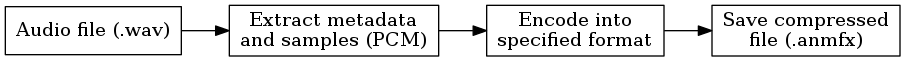
\includegraphics[width=\textwidth]{design_encoder.png}
\end{figure}

Next, each format's encoding process will be outlined (third step in the figure). If the audio file has multiple channels, this process is repeated on each channel separately.

\subsection{ANMF-RAW}
\begin{figure}[ht]
	\caption[ANMF-RAW Encoder]{The encoding scheme for ANMF-RAW.}
	\label{fig:encoding_nmf_raw}
	\centering
	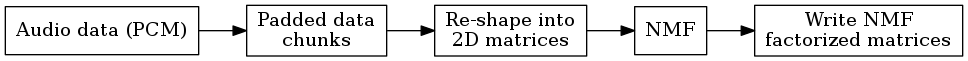
\includegraphics[width=\textwidth]{nmf_raw.png}
\end{figure}

ANMF-RAW works on the principle of applying NMF directly to the PCM audio samples $x_n$. However, the samples are initially an array of 16-bit signed integers, and as such, they need to be processed first before NMF can be used.

A chunk shape is specified to determine how many rows and columns each matrix will have before NMF. We choose a target matrix shape of $1152 \times 200$ to match the amount of samples per frame in the other methods.The sample array is then padded with zeroes to ensure there are enough elements at the end of the array to ensure every matrix can have the same shape and number of elements. The amount of padding must be written to the output so that we know the length of the original array when decoding.

Once the array is padded, we iterate over the samples and split them into equal chunks of size $rows*columns$. This array is then "folded" to produce a matrix of the desired shape. We then obtain a matrix of signed integers, so in order to be able to use NMF, we first need to get rid of all the negative values. To do that, we increment each chunk by the absolute value of its smallest element, guaranteeing that the lowest value in the matrix is $\ge 0$.

Once we have this matrix, we proceed by applying basic random-initialized Euclidean-based NMF on it, obtaining the basis matrix $W$ and coefficient matrix $H$. Lastly, for each chunk, we write the value we incremented the matrix by, and the two decomposition matrices.

\begin{table}[htbp]\caption{ANMF-RAW data structure}
	\label{tab:anmf_raw_file}
	\centering
	\begin{tabular}{|c|c|l|}
		\hline
		Bytes (relative) & Data type & Description \\ \hline
		0-3 & uint32 & amount of zeroes used to pad the samples \\
		4-7 & uint32 & amount of chunks \\
		8-? & data\_chunk[] & NMF-compressed data chunks (refer to Table \ref{tab:anmf_raw_data}) \\
		\hline
	\end{tabular}
\end{table}

\begin{table}[htbp]\caption{ANMF-RAW structure of each data chunk}
	\label{tab:anmf_raw_data}
	\centering
	\begin{tabular}{|c|c|l|}
		\hline
		Bytes (relative) & Data type & Description \\ \hline
		0-7 & float64 & absolute value that the matrix was incremented by \\
		8-? & matrix(float32) & matrix $W$ \\
		?-? & matrix(float32) & matrix $H$ \\
		\hline
	\end{tabular}
\end{table}

\subsection{ANMF-MDCT}
\begin{figure}[ht]
	\caption[ANMF-MDCT Encoder]{The encoding scheme for ANMF-MDCT.}
	\label{fig:encoding_nmf_mdct}
	\centering
	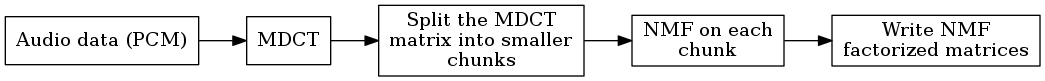
\includegraphics[width=\textwidth]{nmf_mdct.png}
\end{figure}

In ANMF-MDCT, as the name suggests, the PCM input will be transformed using MDCT as per Section \ref{sec:mdct}. Since this is a lapped transform, each transformed block will have a 50\% overlap with the following block. We choose a frame size of $2N = 1152$ and split the signal into blocks of that size, thus each block will contain $N = 576$ coefficients from its own block, and another $576$ from the following one.

The decision to have a block size of $N = 576$ stems from the fact that this will give us the same amount of frequency resolution that e.g. MP3 uses (as seen in Section \ref{sec:mp3}), which proved to be enough for human hearing.

As before, we first pad the signal at the end with zeroes to align it to the desired block size. To prevent loss of data in the first and the last block due to the overlapping, we further pad the signal by an array of zeroes, equal in size to the size of a block, that is $N$ zeroes both at the beginning and the end of the signal.

Then, we apply a windowing function on each block to bring the values near the edges closer to $0$ to help mitigate spectral leakage. We use the MLT window $w_n^M$ as defined in Section \ref{sec:mlt}.

Finally, we apply the MDCT on each of the windowed blocks and obtain a matrix of MDCT coefficients in the form of real numbers.

This matrix is then split into smaller chunks. For example, if the MDCT matrix contains $576$ rows and $1100$ columns, we might split it into submatrices sized $576 \times 200$, with the last one being $576 \times 100$, as no padding is necessary here. This amount of chunks is written to the output. Basic random-initialized Euclidean-based NMF is then ran on each of the chunks separately and the decomposition matrices serialized.

\begin{table}[htbp]\caption{ANMF-MDCT data structure}
	\label{tab:anmf_mdct_file}
	\centering
	\begin{tabular}{|c|c|l|}
		\hline
		Bytes (relative) & Data type & Description \\ \hline
		0-3 & uint32 & amount of zeroes used to pad the samples \\
		4-7 & uint32 & amount of MDCT submatrix chunks \\
		8-? & data\_chunk[] & NMF-compressed MDCT chunks (refer to Table \ref{tab:anmf_mdct_data}) \\
		\hline
	\end{tabular}
\end{table}

\begin{table}[htbp]\caption{ANMF-MDCT structure of each data chunk}
	\label{tab:anmf_mdct_data}
	\centering
	\begin{tabular}{|c|c|l|}
		\hline
		Bytes (relative) & Data type & Description \\ \hline
		0-7 & float64 & absolute value that the matrix was incremented by \\
		8-? & matrix(float32) & matrix $W$ \\
		?-? & matrix(float32) & matrix $H$ \\
		\hline
	\end{tabular}
\end{table}

\subsection{ANMF-STFT}
\begin{figure}[ht]
	\caption[ANMF-STFT Encoder]{The encoding scheme for ANMF-STFT.}		\label{fig:encoding_nmf_stft}
	\centering
	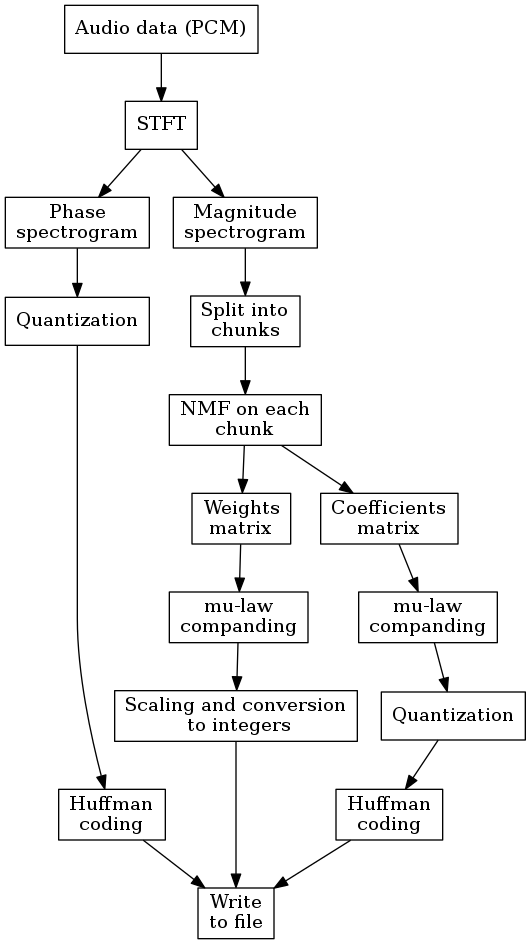
\includegraphics[width=0.6\textwidth]{nmf_stft.png}
\end{figure}

The design of ANMF-STFT is based on the solution suggested in \cite{nikunen_2010} with some changes along with only utilizing open source solutions.

Like with ANMF-MDCT, we choose a frame size of $N = 1152$, leading to a frequency resolution of $576$ bins. We begin by properly padding the signal to $N$ so that it's possible to be split into equal parts. We then use STFT with 50\% overlap and a block size of $N$, which means we end up with twice the coefficients compared to MDCT, but this is not a major issue.

During STFT, we must again window each block, leading to overlapping windows. We use the Hann window $w_n^H$ for this (as defined in Section \ref{sec:hann}).

Once STFT is finished, we end up with a matrix of Fourier transform coefficients in the form of complex numbers. Trying to apply NMF on the complex numbers directly would yield similar results to ANMF-MDCT, so we have to approach this differently.

If we visualise the complex valued elements in the complex plane, we can instead represent each element $z$ as two separate values:

\begin{description}
	\item[magnitude] also called the modulus, geometrically it's the distance from 0
	\item[phase] also called the argument, geometrically it's the angle from the real axis
\end{description}

To obtain the phase $\phi$ of a complex number $z = x + iy$, we can use the following formula:

\begin{align}
\phi(z) = \arg(z) = \arctantwo(y,x)
\end{align}

And to obtain the magnitude $|z|$ of the complex number:

\begin{align}
|z| = \sqrt{x^2 + y^2}
\end{align}

By calculating the magnitude and phase of every element in the STFT matrix individually, we obtain the magnitude spectrogram and the phase spectrogram respectively. We now need to encode both of them individually.

For the phase matrix, my experiments showed that applying NMF on it leads to a very noticeable loss in quality, so instead I opted for a different solution that ultimately ends up saving more space than NMF would.

The phase matrix contains values ranging from $-\pi$ to $\pi$. These values are uniformly quantized into 8 levels ($n_p = 3$ bits) as per Section \ref{sec:unif_quant}. Due to the relative frequency of the boundary values $-\pi$ and $\pi$, a mid-tread quantizer is used. The frequency of each quantization level is visible in Figure \ref{fig:stft_phase_quant_freq}.

Using these frequencies, we are able to then construct a Huffman coding table (refer to Section \ref{sec:huffman}) and use it to losslessly encode the quantized phase matrix using at most 4 bits per value.

\begin{figure}[ht]
	\caption[ANMF-STFT quantized phase frequencies]{Frequency of each quantization level in the phase spectrogram. Data taken from the average of all the example audio files.}
	\label{fig:stft_phase_quant_freq}
	\centering
	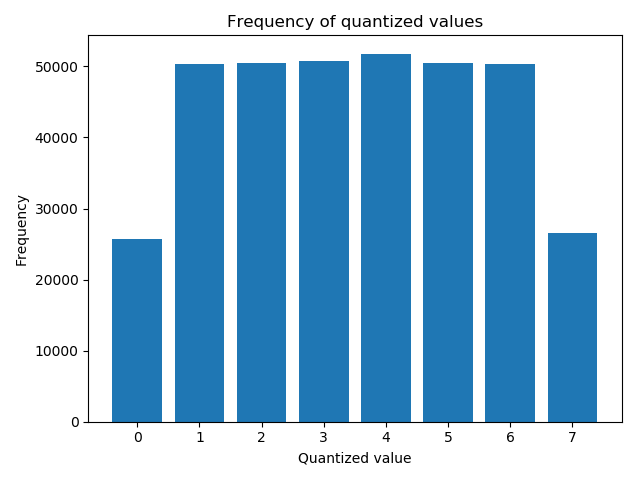
\includegraphics[width=\textwidth]{stft_phase_quant_freq.png}
\end{figure}

The magnitude spectrogram is where we actually use NMF. As it is effectively a matrix of signal amplitudes, it's less prone to noticeable quality loss if the values deviate a little. We split the magnitude matrix column-wise into smaller submatrices, e.g. $chunk_size = 500$.

On each submatrix we then run basic random-initialized Euclidean-based NMF, obtaining the weight matrix $W$ and coefficient matrix $H$.

For the next step, we apply $\mu$-law compression to both the decomposition matrices, as defined in Section \ref{sec:mulaw}. In order to be able to do that, we first scale both matrices to the range $[0, 1]$. We do this by applying the following formula to all elements in both matrices:

\begin{align}
M'_{ij} = \frac{M_{ij} - \min(M)}{|\max(M) - \min(M)|}
\end{align}

To restore the original scale later, we need to save both the minimum and maximum value, otherwise they will be lost in the non-uniform quantization.

For the $\mu$-law compression, we experiment with the value of $\mu$ later, but a good start is $\mu_W = 10^4$ and $\mu_H = 10^5$. We do this because we want to lower the amount of bits needed to represent each value, without losing the values near zero - that would lead to a large loss of quality, or in some cases, loss of the signal itself.

In the weight matrix, we then convert the compressed values into 32-bit unsigned integers, as going to values below that proved to cause loss of signal data, and this integer matrix is then serialized into the file.

However, in the case of the coefficient matrix $H$, we can go a lot further. We use a uniform quantizer with 32 levels ($n_h = 5$ bits) and we opt for a mid-tread quantizer again, as we want to be able to reconstruct a value of $0$, i.e. feature not present.

Similarly to the phase matrix, we take these quantized values and look at their frequencies. The results of this analysis are visible on Figure \ref{fig:stft_quant_freq}.

\begin{figure}[ht]
	\caption[ANMF-STFT quantized magnitude coefficient frequencies]{Frequency of each quantization level in the decomposed coefficients matrix of the magnitude spectrogram. Data taken from the average of all the example audio files.}
	\label{fig:stft_quant_freq}
	\centering
	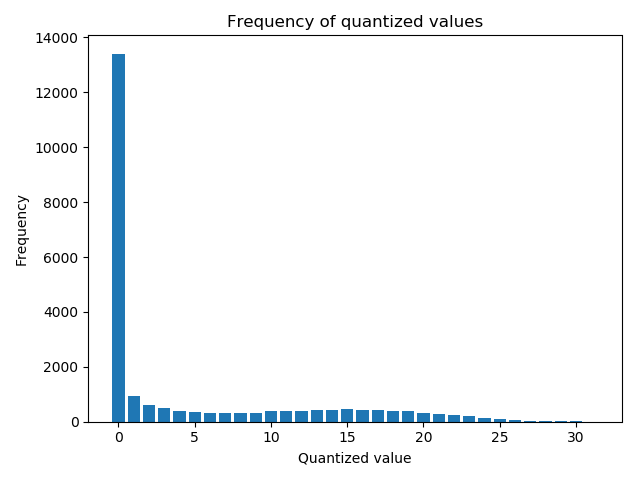
\includegraphics[width=\textwidth]{stft_quant_freq.png}
\end{figure}

Using this information, we can construct another Huffman coding table, separate for this matrix. As we can see, even despite the $\mu$-law compression, a lot of values still fall to a quantized value of $0$.

In a Huffman table from these frequencies, we then assemble the shortest code to the value $0$, i.e. we only need 1 bit. The longest code in a table constructed this way for 32 levels of quantization will only require 11 bits. Overall, we save a lot of space saving the matrix this way as opposed to storing the values as 32-bit floats or integers.

\begin{table}[htbp]\caption{ANMF-STFT data structure}
	\label{tab:anmf_stft_file}
	\centering
	\begin{tabular}{|c|c|l|}
		\hline
		Bytes (relative) & Data type & Description \\ \hline
		0-3 & uint32 & amount of zeroes used to pad the samples \\
		4-7 & uint32 & amount of STFT submatrix chunks \\
		8-? & quant\_matrix & quantized phase matrix \\
		?-? & data\_chunk[] & NMF-compressed magnitude chunks (refer to Table \ref{tab:anmf_stft_data}) \\
		\hline
	\end{tabular}
\end{table}

\begin{table}[htbp]\caption{ANMF-STFT structure of each magnitude submatrix}
	\label{tab:anmf_stft_data}
	\centering
	\begin{tabular}{|c|c|l|}
		\hline
		Bytes (relative) & Data type & Description \\ \hline
		0-7 & float64 & absolute value that the matrix was incremented by \\
		8-15 & float64 & minimum value before scaling to $[0, 1]$ \\
		16-23 & float64 & maximum value before scaling to $[0, 1]$ \\
		24-? & matrix(uint32) & $\mu$-law compressed matrix $W$ \\
		?-? & quant\_matrix & quantized $\mu$-law compressed matrix $H$ \\
		\hline
	\end{tabular}
\end{table}

\subsubsection{Huffman encoding}
\label{sec:huffman}
Huffman code refers to an optimal prefix coding scheme often employed for lossless compression. It's used to compress a message that only consists of members from a finite, known beforehand set of symbols. \cite{huffman_1952}

The goal is to create a dictionary that maps each value to a sequence of bits, where none of the sequences is a prefix of another one, which means that there are no ambiguities when decoding a Huffman encoded message, and we do not need to store any information about where one code begins and where it ends.

The main characteristic of a Huffman code is that the more frequent a symbol is, the shorter code it will be assigned. So in the case of a system where a certain symbol is very frequent, a message consisting of mostly those symbols will be compressed greatly, with no loss of data.

\begin{algorithm}[h]
\caption{Huffman code compression}
\label{alg:huffman}
\KwIn{a list of symbols and their probabilities}
\KwOut{a Huffman tree}
queue $\leftarrow$ new PriorityQueue()\;
\ForEach{item x in input}{
	node $\leftarrow$ new Node()\;
	node.symbol $\leftarrow$ x.symbol\;
	node.prob $\leftarrow$ x.probability\;
	node.leftChild, node.rightChild $\leftarrow$ null\;
	queue.enqueue(node, node.prob)\;
}
\While{queue.length $>$ 1}{
	node1 $\leftarrow$ queue.dequeue()\;
	node2 $\leftarrow$ queue.dequeue()\;
	newNode $\leftarrow$ new Node()\;
	newNode.leftChild $\leftarrow$ node1\;
	newNode.rightChild $\leftarrow$ node2\;
	newNode.prob $\leftarrow$ node1.prob + node2.prob\;
	queue.enqueue(newNode, newNode.prob)\;
}
\end{algorithm}

Algorithm \ref{alg:huffman} describes the compression process, at the end of which we obtain a Huffman tree. By traversing this tree from the root and assigning every left child a $0$ and every right child a $1$ and concatenating these bits as we reach the symbols in the leafs, we obtain the Huffman code for the given symbol. The asymptotic complexity of this algorithm is $\mathcal{O}(n \log n)$, essentially we need $\mathcal{O}(\log n)$ time to determine the highest priority in the queue, and there are $\mathcal{O}(n)$ iterations.

Often, the dictionary itself has to be encoded as well, but as the frequencies are roughly the same for each audio file, the tree can be fixed directly into the implementation.

\section{Decoder}
Similar to the encoder, the decoder simply reverses the encoding process as seen in Figure \ref{fig:design_decoder}. As this process is fairly straightforward for each of the methods, it won't be elaborated on further.

\begin{figure}[ht]
	\caption[Decoder overview]{A high level overview of the ANMF audio decoder.}
	\label{fig:design_decoder}
	\centering
	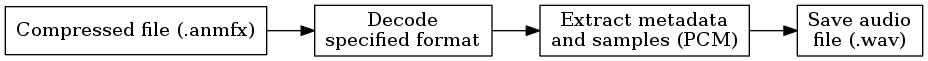
\includegraphics[width=\textwidth]{design_decoder.png}
\end{figure}


\chapter{Implementation}
This chapter will explain the specific details of implementing the audio codec outlined in the previous chapter.

\section{Encoder}
.. process of encoding ..

\subsection{NMF-RAW}
TODO

\subsection{NMF-MDCT}
TODO describe MDCT as transformed DCT-IV (mdct.py)

\subsection{NMF-STFT}

.. application of NMF ..

.. variables ..

\section{Decoder}

\chapter{Evaluation}
In this section you will find an evaluation of the different algorithms, including experiments with various parameters for them and comparison to existing solutions from Section \ref{sec:stateoftheart}.

\section{Methodology}
Audio compression quality is most often evaluated using a series of listening tests (such as the one pictured in Figure \ref{fig:opus_listening_test}). However, due to a lack of resources to conduct such a thing, a different method must be used - although they are generally not as accurate.

One of the most used methods for objectively evaluating perceptible audio quality is PEAQ \cite{peaq_2006}, however its specifications are insufficient, and its implementations proprietary. The exact algorithm and parameters aren't known for the most part. It comes in two variants:

\begin{description}
	\item[PEAQ Basic] intended for real-time use
	\item[PEAQ Advanced] a more comprehensive model, intended for non real-time use
\end{description}

Even though neither of these is directly available, luckily, there are a few open-source alternatives that try to implement similar algorithms, with their quality measured by comparing their output to PEAQ, and by proxy, to listening tests.

One of the more prominent open-source solutions is GstPEAQ, which according to its paper \cite{gstpeaq_paper} performs better than the other implementations. So while it does not conform to the PEAQ recommendation directly, its results are within an acceptable margin and thus this thesis will use GstPEAQ for quality evaluation.

\section{GstPEAQ}
GstPEAQ is a plugin for GStreamer \cite{gstreamer_2016} (a pipeline-based multimedia framework) and its source code is freely available at \cite{gstpeaq_impl}. It implements both the Basic and Advanced mode of PEAQ as specified in \cite{peaq_2006}, however as the standard is under-specified, educated guesses must be taken at points.

And just like PEAQ, the algorithm's main output is a value known as \emph{Objective Difference Grade} (ODG), which evaluates the perceptible impairment (quality difference) between the provided audio and the reference audio. It uses various psychoacoustic "features" of the signal to determine the grade, the details of which won't be covered here - please refer to either paper for specifics.

The ODG scale contains real values from $0$ to $-4$, ranging from imperceptible difference to very annoying for the human ear. Please refer to Table \ref{tab:odg_scale} to see the full scale.

\begin{table}[htbp]\caption{PEAQ - Objective Difference Grade table}
	\label{tab:odg_scale}
	\centering
	\begin{tabular}{|c|l|}
		\hline
		ODG & Impairment description \\ \hline
		$0.0$ & Imperceptible \\
		$-1.0$ & Perceptible, but not annoying \\
		$-2.0$ & Slightly annoying \\
		$-3.0$ & Annoying \\
		$-4.0$ & Very annoying \\
		\hline
	\end{tabular}
\end{table}

\section{Evaluating results}
In this section we will experiment with various parameters for all the encoding methods, find a good compromise between bitrate and ODG, and then compare those results to the reference codings (MP3, Opus) at similar bitrates.

The evaluating process will work in these steps:

\begin{enumerate}
	\item compress example WAV file using ANMF
	\item decompress ANMF back to a WAV file
	\item measure ODG between old and new WAV file
\end{enumerate}

In the case of MP3 or Opus files, they will be decoded to WAV for comparison.

\subsection{Audio examples}
There's a total of four example audio files in WAV format that will be used for testing. Please refer to Table \ref{tab:audio_examples} for a list. All of the examples are $\sim5-10$ second excerpts from audio files using 44.1 kHz sampling rate and 16-bit signed integer samples. These files can be found in the \verb|examples| folder of the implementation.

\begin{table}[htbp]\caption{List of tested audio files}
	\label{tab:audio_examples}
	\centering
	\begin{tabular}{|c|c|c|c|l|}
		\hline
		ID & File name & Description \\ \hline
		$00$ & \verb|piano16t.wav| & Clear sounding piano sounds \\
		$01$ & \verb|henry16t.wav| & Average quality English voice \\
		$02$ & \verb|swave16t.wav| & Simple electronic music \\
		$03$ & \verb|taleena16t.wav| & Complex music including lyrics \\
		\hline
	\end{tabular}
\end{table}

\subsection{Bitrate}
The bitrate is the amount of bits that a computer needs to process per a unit of time, in this context it means how many bits are needed to play back 1 second of an audio file.

To find the bitrate of a WAV file, we can use the following equation:

\begin{align}
bitrate = channelCount \cdot samplingRate \cdot bitsPerSample
\end{align}

So in regards to compressing the example files, our target bitrate is at most $2 \cdot 44100 \cdot 16 = 1411200$ bits per second (or $\sim 1411$ kbps).

To calculate the number of elements in an NMF-approximated matrix $V$ of size $m \times n$ with approximation rank $r$, we can use the following equation:

\begin{align}
\label{equ:nmf_size}
size(NMF(V)) = r(m+n)
\end{align}

\emph{Proof:} NMF approximates a matrix $m \times n$ into two matrices $m \times r$ and $r \times n$, therefore the total size is $mr + rn = r(m+n)$.

\subsection{ANMF-RAW}
For ANMF-RAW, we need to find a compromise between the size of one chunk and the rank of the NMF. First, we'll fix the shape to $1152 \times 200$ and experiment with the rank.

The maximum number of iterations has been fixed to 3000, since past that point the cost function is almost stable as seen in Figure \ref{fig:anmf_raw_cost_func}.

\begin{figure}[ht]
	\caption[ANMF-RAW cost function]{The value of the cost function per iteration during NMF in ANMF-RAW at rank $= 30$.}
	\label{fig:anmf_raw_cost_func}
	\centering
	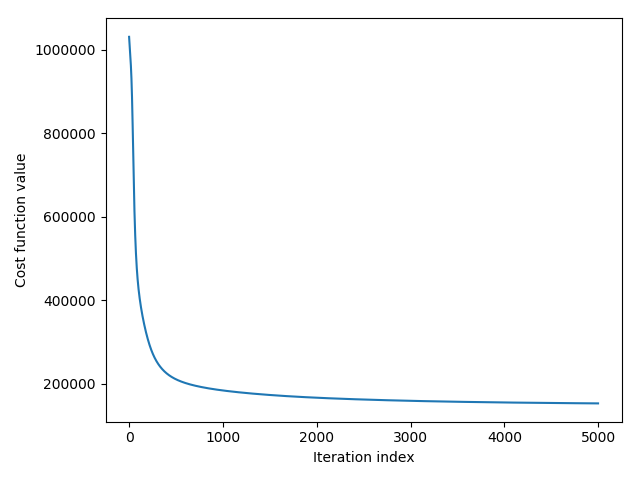
\includegraphics[width=\textwidth]{anmf_raw_cost_func.png}
\end{figure}

In Table \ref{tab:anmf_raw_rank}, you can see the results of changing the rank of the NMF approximation. The rows correspond to the example IDs from Table \ref{tab:audio_examples}, and the columns correspond to the ODG for different rank values.

\begin{table}[htbp]\caption{ANMF-RAW rank experiment results}
	\label{tab:anmf_raw_rank}
	\centering
	\begin{tabular}{|c|c|c|c|c|c|}
		\hline
		ID & rank 30 & rank 40 & rank 45 & rank 60 & rank 75 \\ \hline
		$00$ & $-3.873$ & $-3.830$ & $-3.811$ & $-3.749$ & $-3.650$ \\
		$01$ & $-3.908$ & $-3.902$ & $-3.895$ & $-3.861$ & $-3.844$ \\
		$02$ & $-3.868$ & $-3.850$ & $-3.837$ & $-3.800$ & $-3.759$ \\
		$03$ & $-3.744$ & $-3.519$ & $-3.361$ & $-2.825$ & $-2.461$ \\		
		\hline
	\end{tabular}
\end{table}

It's also worth mentioning that the runtime necessary for compression scales with the rank, as seen in Table \ref{tab:anmf_raw_runtime}.

\begin{table}[htbp]\caption{ANMF-RAW average runtime in seconds}
	\label{tab:anmf_raw_runtime}
	\centering
	\begin{tabular}{|c|c|c|c|c|c|}
		\hline
		ID & rank 30 & rank 40 & rank 45 & rank 60 & rank 75 \\ \hline
		$00$ & $63.378$s & $65.913$s & $67.082$s & $71.684$s & $75.839$s \\	
		\hline
	\end{tabular}
\end{table}

Interestingly enough, sample ID 03 notices the largest improvement despite being the more complex of the four, but when listening to the decompressed audio, it still sounds quite distorted and noticeable. Another looming issue is that at that rank the size of the compressed file approaches the original filesize, so we will need to lower the rank and try a lower chunk size instead.

To calculate the bitrate of ANMF-RAW, we must take into account the chunk size and the rank of the NMF approximation and then use Equation \ref{equ:nmf_size}. There is some overhead for the metadata, but as it spans only a few bytes it will be disregarded. The bitrate of ANMF-RAW with a chunk size of $m \times n$ and rank $r$ can be calculated as:

\begin{align}
bitrate^R = r(m+n) \cdot \frac{sampleRate}{mn} \cdot bitsPerValue \cdot channelCount
\end{align}

Therefore, for a chunk $1152 \times 200$ with rank 75, we get:

\begin{align}
bitrate^R = 75 \cdot (1152 + 200) \cdot \frac{44100}{1152 \cdot 200} \cdot 32 \cdot 2 = 1242150
\end{align}

Our target is 1411 kbps and our compression with 1242 kbps is judged as "annoying" by GstPEAQ. We will try lowering the chunk size and rank both to see if it has an effect. It was mentioned in Section \ref{sec:mp3} that it can compress music by up to a factor of 12 without noticeable loss in quality. Here, with this method, we are going to aim for at least around half that.

We take a rank of 40 and a target bitrate of 750 kbps. We pick e.g. $600$ for $m$ and solve the equation above, obtaining $n = 200$. However, when trying out these new parameters, the ODG barely changed from the previous shape, and further testing of this method was thus stopped due to unsatisfactory results.

\subsection{ANMF-MDCT}
.. TODO experiment with parameters and calculate bitrate ..

\subsection{ANMF-STFT}
.. TODO experiment with parameters and calculate bitrate ..

\subsection{Comparison}
.. TODO calculate bitrate for the wav files ..
.. TODO compare the "best" from the previous 3 vs MP3/Opus ..


\setsecnumdepth{part}
\chapter{Conclusion}
.. what went right ..


.. what went wrong ..


.. what could be improved ..
add psychoacoustics
try compressing LPC/SILK


\bibliographystyle{iso690}
\bibliography{mybibliographyfile}

\setsecnumdepth{all}
\appendix

\chapter{Acronyms}
\begin{description}
	\item[todo] TODO
\end{description}


\chapter{Contents of enclosed CD}

\begin{figure}
	\dirtree{%
		.1 readme.txt\DTcomment{the file with CD contents description}.
		.1 exe\DTcomment{the directory with executables}.
		.1 src\DTcomment{the directory of source codes}.
		.2 wbdcm\DTcomment{implementation sources}.
		.2 thesis\DTcomment{the directory of \LaTeX{} source codes of the thesis}.
		.1 text\DTcomment{the thesis text directory}.
		.2 thesis.pdf\DTcomment{the thesis text in PDF format}.
		.2 thesis.ps\DTcomment{the thesis text in PS format}.
	}
\end{figure}

\end{document}
